\documentclass{standalone}
\usepackage{pgfplots}
\usetikzlibrary{arrows}

\begin{document}
  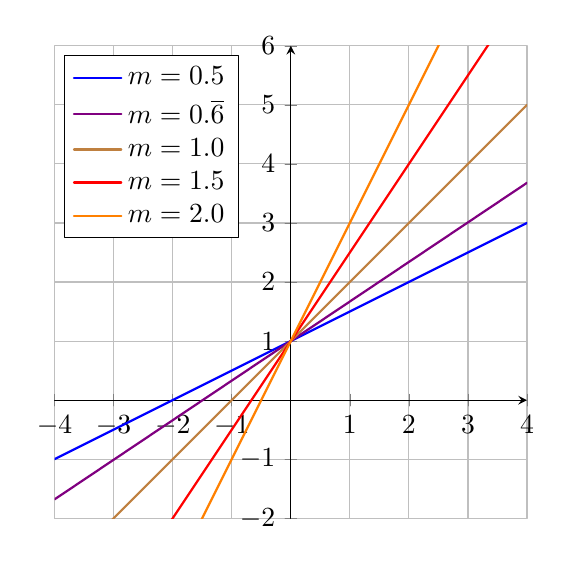
\begin{tikzpicture}[line cap=round,line join=round,>=triangle 45]
    \begin{axis}[
      x=0.75cm,y=0.75cm,
      axis lines=middle,
      ymajorgrids=true,
      xmajorgrids=true,
      xmin=-4,
      xmax=4,
      ymin=-2,
      ymax=6,
      xtick={-4,-3,...,4},
      ytick={-2,-1,...,6},
      legend style={at={(0.02,0.98)},anchor=north west}
      ]
      \addplot [mark=none,samples=200,thick,blue,domain=-4:4] {0.5*x+1};
      \addplot [mark=none,samples=200,thick,violet,domain=-4:4] {0.67*x+1};
      \addplot [mark=none,samples=200,thick,brown,domain=-4:4] {(1*x)+1};
      \addplot [mark=none,samples=200,thick,red,domain=-4:4] {(1.5*x)+1};
      \addplot [mark=none,samples=200,thick,orange,domain=-4:4] {(2*x)+1};
      \legend{$m=0.5$, $m=0.\overline{6}$, $m=1.0$, $m=1.5$, $m=2.0$}
    \end{axis}
  \end{tikzpicture}
\end{document}
